\documentclass[10pt,a4paper]{article}

\usepackage[utf8]{inputenc}
\usepackage[francais]{babel}
\usepackage[T1]{fontenc}
\usepackage{amsmath}
\usepackage{amsfonts}
\usepackage{amssymb}
\usepackage{graphicx}
\usepackage{lmodern}
\usepackage{hyperref}
\usepackage[left=3cm,right=3cm,top=2cm,bottom=3cm]{geometry}

\title{Guide d'installation OTB\\
  {\small\url{https://www.orfeo-toolbox.org}}
}

\begin{document}

\maketitle

\section{Windows}

\subsection{QGIS}
Installer QGIS: \url{http://www.qgis.org/fr/site/forusers/download.html}.
\subsection{(Optionnel) Ligne de commande}
Installer un environnement minimal de ligne de commande pour Windows. Par exemple
Git for Windows est très facile à installer:
\url{http://git-scm.com/download/win}.

\subsection{OTB et Monteverdi}
Pour installer OTB 5.2.1 et Monteverdi 3.0.1, télécharger les paquets
correspondants à votre architecture (32 ou 64 bits). Si votre machine est 32
bits:

\begin{verbatim}
Monteverdi-3.0.1-win32.zip
OTB-5.2.1-win32.zip
\end{verbatim}

Sinon si votre machine est 64 bits:

\begin{verbatim}
Monteverdi-3.0.1-win64.zip
OTB-5.2.1-win64.zip
\end{verbatim}

Ces archives sont disponibles sur \url{https://www.orfeo-toolbox.org/packages/}.
Extraire les deux archives zip dans votre répertoire personnel, par exemple dans:\\
\begin{centering}
\texttt{C:{\textbackslash}Utilisateurs{\textbackslash}Martin{\textbackslash}install{\textbackslash}}.
\end{centering}

\subsection{Tester l'installation}
Une fois l'installation terminée, les applications OTB sont accessibles de
plusieurs façons:
\begin{enumerate}

  \item Lancer monteverdi en navigant dans le dossier \texttt{bin} de son répertoire
d'installation, par exemple:
\texttt{Martin{\textbackslash}install{\textbackslash}Monteverdi-3.0.1-win32{\textbackslash}bin},
puis double cliquer sur \textbf{\texttt{monteverdi.bat}} (et non pas
\texttt{monteverdi.exe}).
Puis charger les applications OTB avec "Fichier" $\rightarrow$ "Charger les
OTB-Applications".
Le navigateur d'application est ensuite accessible depuis "Affichage"
$\rightarrow$ "Navigateur d'OTB-Applications".
(Voir figure \ref{fig:windows-mapla}).

  \item Naviguer dans le dossier \texttt{bin} du répertoire d'installation OTB et double cliquer sur le
  fichier \texttt{.bat} de l'application à lancer, par exemple:\\
  \texttt{Martin{\textbackslash}install{\textbackslash}OTB-5.2.1-win32{\textbackslash}bin{\textbackslash}otbgui\_Rescale.bat}
  (Voir figure \ref{fig:windows-otbgui}).

  \item Ouvrir une ligne de commande, puis taper:

    Pour \texttt{cmd.exe}: \texttt{otbcli\_Rescale.bat -version}

    Pour bash: \texttt{cmd //c otbcli\_Rescale.bat -version}

    Voir figure \ref{fig:windows-otbcli}.

\end{enumerate}

\begin{figure}[h]
  \center
  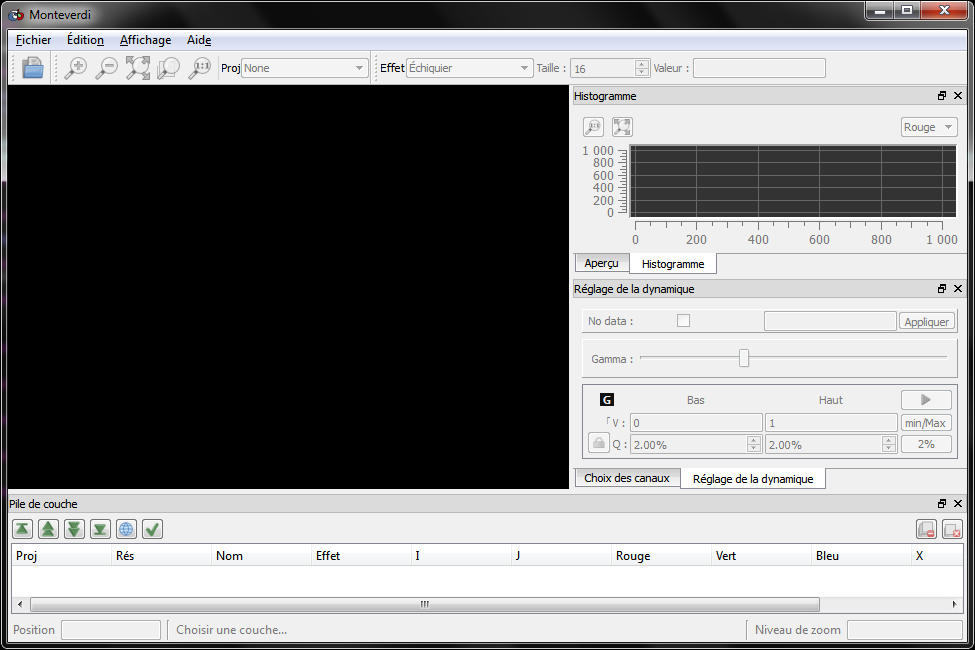
\includegraphics[width=1\textwidth]{Art/windows-monteverdi.png}
  \caption[]{Monteverdi}
  \label{fig:windows-monteverdi}
\end{figure}

\begin{figure}[h]
  \center
  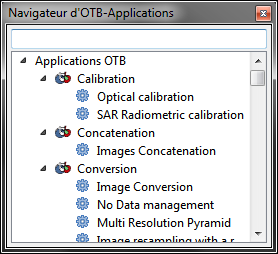
\includegraphics[scale=1]{Art/windows-mapla.png}
  \caption[]{Les applications OTB sont accessibles depuis Monteverdi}
  \label{fig:windows-mapla}
\end{figure}

\begin{figure}[h]
  \center
  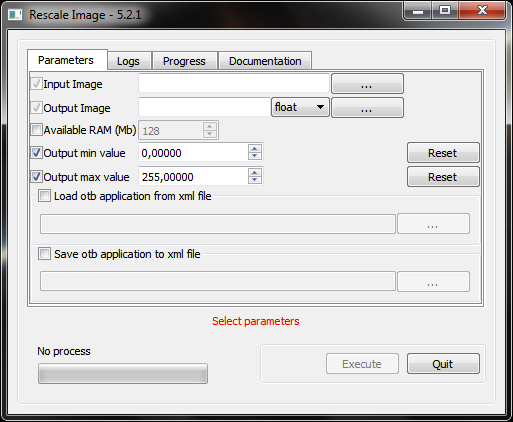
\includegraphics[scale=1]{Art/windows-otbgui.png}
  \caption[]{Interface graphique OTB}
  \label{fig:windows-otbgui}
\end{figure}

\begin{figure}[h]
  \center
  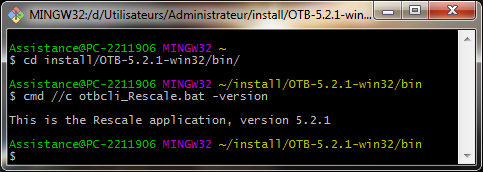
\includegraphics[scale=1]{Art/windows-otbcli.png}
  \caption[]{Ligne de commande OTB}
  \label{fig:windows-otbcli}
\end{figure}

\subsection{OTB depuis QGIS}

Les applications OTB sont disponibles depuis QGIS. Pour cela

Attention ! QGIS est livré avec ses propres binaires OTB. Les applications ainsi
ouvertes depuis QGIS sont souvent différentes de celles installée ci-dessus, car
il s'agit typiquement d'une version plus ancienne.
Éventuellement, il est possible de remplacer l'OTB livrée avec QGIS en supprimant
ou écrasant les fichiers dans \texttt{}.

\begin{figure}[h]
  \center
  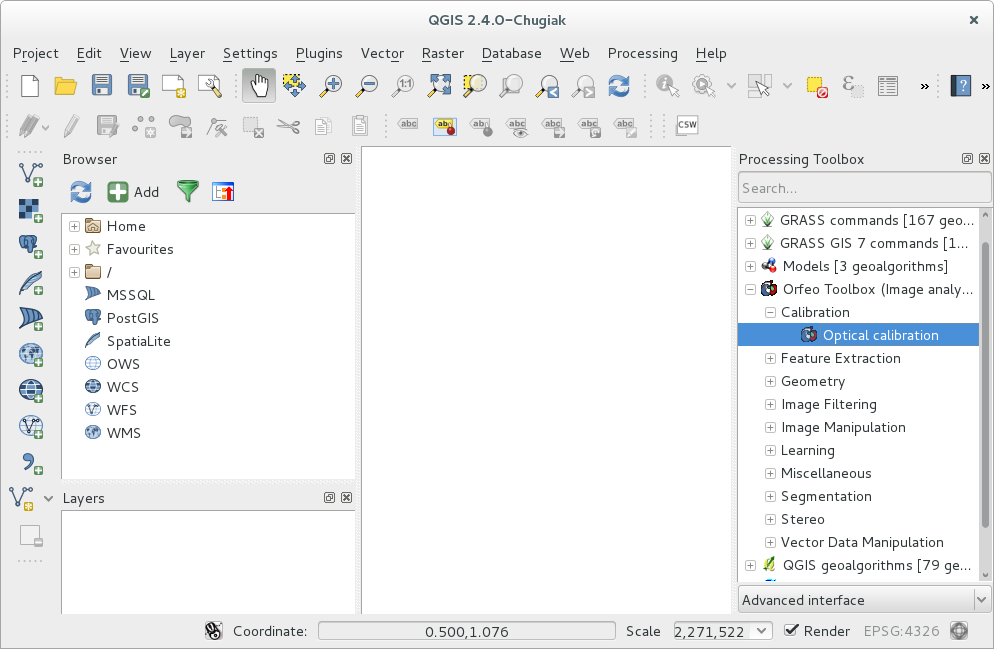
\includegraphics[width=1\textwidth]{Art/qgis-otb.png}
  \caption[]{Intégration QGIS - OTB}
  \label{fig:otb-qgis}
\end{figure}

\clearpage
\section{Ubuntu}

\end{document}
